
The initial $100\times100$ subregion of M2 considered in our main paper was located at pixel coordinates (630, 310) in SDSS run 2583, field 136, camera column 6. 
We evaluate StarNet on two other subregions of M2.
The first is another $100\times100$ pixel subregion of similar density as the original;
the second is in the center of globular cluster
(Figure~\ref{fig:m2_test_regions}).

The performance metrics on the center of the globular cluster 
suggest that deblending in this region is nearly impossible --- there are $15,000$ stars in this $100\times100$ subregion, 
averaging to more than one star per pixel. 

In all the considered regions, our comparison with DAOPHOT is unchanged, and we continue to outperform DAOPHOT in F1 score. 

\begin{figure}[tb]
    \centering
    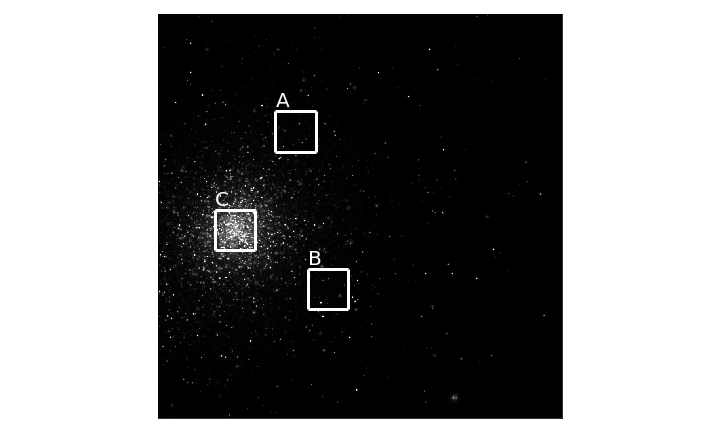
\includegraphics[width=0.6\textwidth]{figures/m2_results/test_images.png}
    \vspace{-0.5cm}
    \caption{Subregions of M2 for the performance metrics in Table~\ref{tab:summary_stats_m2test}. The subregion labeled "A" was cataloged in the main text. 
}
    \label{fig:m2_test_regions}
\end{figure}

\begin{table}[ht]
\centering
\caption{Performance metrics on the M2 test subregion. 
StarNet-init is the network fit on the original M2 subregion (the same network as StarNet-WS in the main text). 
StarNet-refit ran two further wake-sleep cycles on the M2 test subregion. }
\label{tab:summary_stats_m2test}
\begin{tabular}{l|ccc|cc}
\toprule
     Method &   TPR &   PPV &  F1 score &  \#stars & (q-5\%, q-95\%)\\
\midrule
    DAOPHOT &  0.13 &  0.53 &      0.21 &     338 & -- \\
       PCAT &  0.44 &  0.37 &      0.41 &    1793 & (1799, 1805)\\
 StarNet-init &  0.47 &  0.47 &      0.47 &    1466 & (1431, 1499)\\
 StarNet-refit &  0.47 &  0.50 &      0.48 &     1396 & (1362, 1432)\\
     Hubble &  1.00 &  1.00 &      1.00 &     1413 & -- \\
\bottomrule
\end{tabular}
\end{table}


